\documentclass[asme2ejs.tex]{subfiles}

\begin{document}
\section{Methodology}

It is necessary to clearly state our assumptions for the following analysis as many considerations have be approximated or considered on a theoretical basis since the actual effects are quite complex. 
In summary, our assumptions for the various sub-systems of our model require:
\begin{itemize} % System level
	\item Foams
		\begin{itemize}
			\item 	Error introduced by using Kelvin relation is acceptable versus computational effort for W-P structure
			\item	Metal foam measurements are known to be inaccurate. 
			For a foam of 0.97 porosity ($\epsilon$), the Kelvin stucture with a spherical void to yield the given porosity can be optimized to an analytical geometry constructed of spheres and equilateral prisms that is equivalent to a metal foam. 
			[Bhattacharaya 		\& Mahajan 2002 AIAA] state that the limit of the equilateral triangle geometry extends to $\epsilon = 0.94$ before becoming a convex prism. 
			We take this as an error in our model that is reasonable to perform the calculations.
		\end{itemize}

	\item Thermodynamics
		\begin{itemize}
			\item	Constant specific heat ($c_v$)
			\item 	Real fluid properties
			\item 	For a pressure drop along the length of the tube/foam, the saturation temperature also changes with length of the pipe.
		\end{itemize}

\item Flows
	\begin{itemize}
		\item 	Only considering saturated, two phase flow 
		\item 	Inlet conditions are fully developed for the metal foam and non-metal foam cases
		\item 	Flow is turbulent on all length scales: tube and pore [Incropera, de Jager 2013 HTEngr]
		\item 	Stable flow conditions. No transition schemes are modeled on any length scale.
		\item 	Only considering dispersed/bubbly and annular flows since the fluid is not subcooled before entering our analysis and the desired exit quality of the flow is 0.8. 
		Alternatively it could be said that we are not considering any form of dimensionalized intermediate flow regime (slug or churn).
		\item	Two flow analysis methods are viable: homogeneous and separated. 
		Homogeneous is applicable in nucleate boiling regime for dispersed flows and separated is applicable in annular flow.
		\item 	The stable consideration also considers a non-transient increase in vapor velocity with increasing mass fraction of vapor as a consequence of maintaining local saturation pressure and temperature in the vapor region.
		\item 	No fluid entrainment in vapor core for annular flow.
	\end{itemize}

\item Heat Transfer
	\begin{itemize}
		\item 	Inlet temperature for the fluid is at saturation temperature
		\item 	Non-thermal equilibrium is assumed with the foam
		\item 	No bubble confinement  (sub cooled boiling) required in our model since fluid is at Tsat at entrance.
	\end{itemize}
\end{itemize}

The usage of metal foams in the boiler to enhance the heat transfer between the boiler and fluid  would effectively increase the rate at which the steam is produced thereby potentially reducing the length of the boiler.0
The analysis of heat transfer in a metal foam can either be performed using a two energy equation volume averaged or a cell/lattice resolution method.
In the volume averaged method the effective surface area, relative density and effective heat transfer coefficient  are used to calculate the various heat transfer properties required to determine the desired results.
\cite{Du2010}
In the cell resolution method, the unit cell of a metal foam is modeled based on various assumption made about the formation of the cell. 
Lord Kelvin was the first to analyze the problem, and his model can be described as a tetrakaidecahedron, or terminated octahedron.
\cite{Kopanidis2010}
This is the model of choice for our study due to symmetry of the unit cell.
It should be noted that this is not the most accurate unit cell representation; the Weaire-Phelan (WP) structure has been proven to better solve the minimization problem of the intersitial gas bubble formation within metal foams. 
The WP structure has an 8 cell group symmetry due to the use of 2 separate cell types, one of which is a irregular dodecahedron.
The basic structure was taken into consideration was to optimise the heat transfer rate and minimize the heat storage in the metal foam, this is basically done by increasing the surface area to volume ratio.
\cite{Kusner1996}

%%%%%%%%%%%%%%%% begin FIGURE 1 %%%%%%%%%%%%%%%%%%%
\begin{figure}[t]
\begin{center}
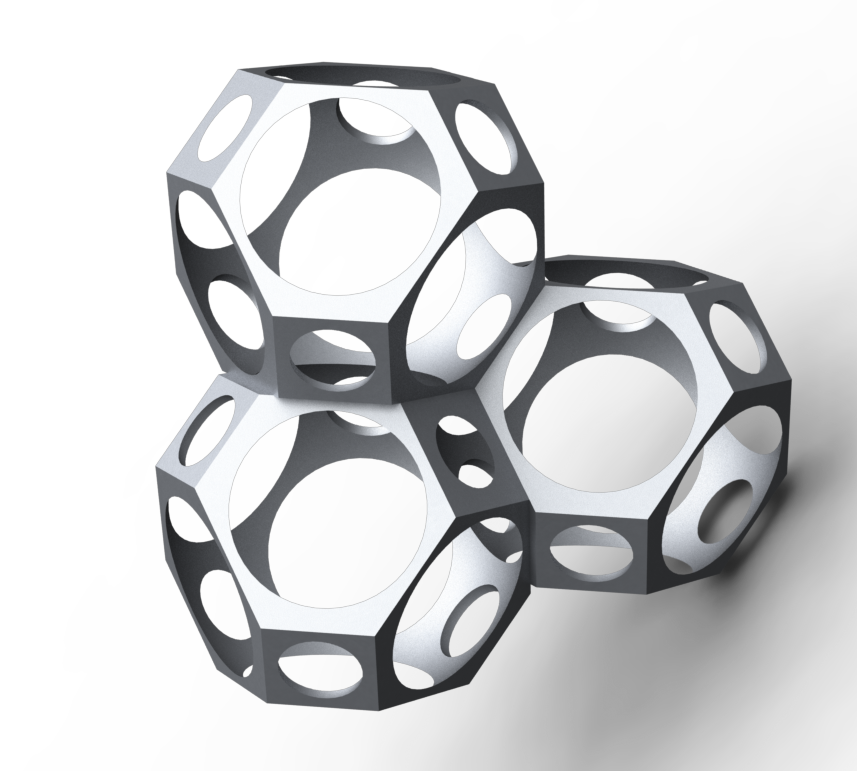
\includegraphics[width=0.35\textwidth]{./figure/CellGroup2}
\end{center}
\caption{Terminated Octahedron also known as a Kelvin Structure}
\label{fig:flowregime}
\end{figure}
%%%%%%%%%%%%%%%% end FIGURE %%%%%%%%%%%%%%%%%%

For our analytical model, we have taken a novel approach to modeling a fin network using the tetrakaidecahedron unit cell as the framework.
To our knowledge, no one has yet published any results using such a method. 
At the nodes, spheres will be placed and for the geometry of the ligaments, isosceles prismatic fins will connect to the spheres. 
A correction factor will be applied to take the sphere contact face as ``flat" to simplify the fin equations. 
Utilizing symmetry, of which the tetrakaidecahedron has symmetry along $90\degree, 120\degree,$ and $180\degree$, it will be determined which symmetry mode will be used to simplify this analytical study.

%%%%%%%%%%%%%%%% begin FIGURE 2 %%%%%%%%%%%%%%%%%%%
\begin{figure}[t]
\begin{center}
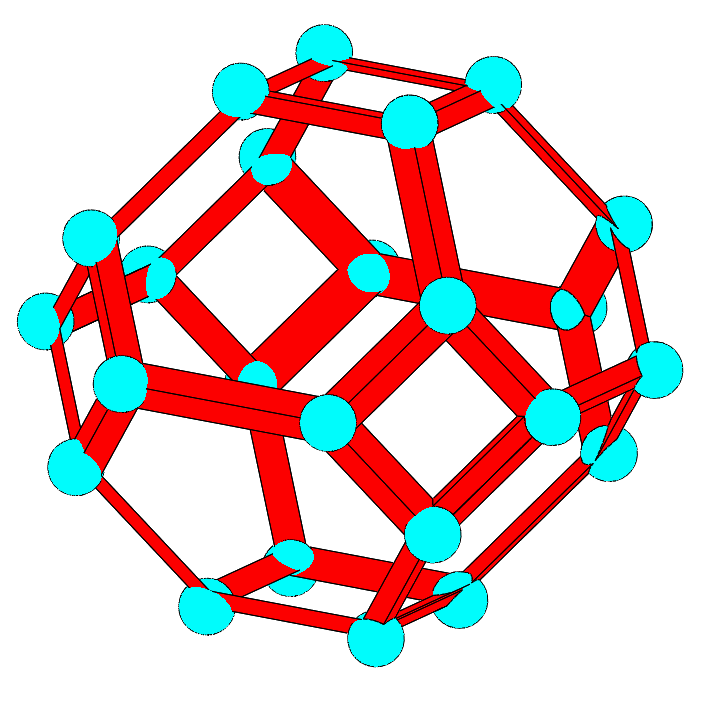
\includegraphics[width=0.35\textwidth]{./figure/Cell_Analytical}
\end{center}
\caption{Analytical fin network with interstitial spheres at nodes}
\label{fig:flowregime}
\end{figure}
%%%%%%%%%%%%%%%% end FIGURE %%%%%%%%%%%%%%%%%%


In either method, the fluids equations are the same, and do not change:

\noindent\textbf{Conservation of Mass}
\begin{equation}
\pdif{u}{x}+\pdif{v}{y} + \pdif{w}{z} = 0
\end{equation}

\textbf{Conservation of Momentum}
\begin{align}
\rho \left( u \pdif{u}{x} + v\pdif{u}{y} + w\pdif{u}{z} \right) &= - \pdif{p}{x} + \mu \left( \podif{u}{x}{2} + \podif{u}{y}{2} + \podif{u}{z}{2} \right) + X\\
\rho \left( u \pdif{v}{x} + v\pdif{v}{y} + w\pdif{v}{z} \right) &= - \pdif{p}{y} + \mu \left( \podif{v}{x}{2} + \podif{v}{y}{2} + \podif{v}{z}{2}  \right) + Y \\
\rho \left( u \pdif{w}{x} + v\pdif{w}{y} + w\pdif{w}{z} \right) &= - \pdif{p}{z} + \mu \left( \podif{w}{x}{2} + \podif{w}{y}{2} + \podif{w}{z}{2}  \right) + Z
\end{align}

Solving the conservation of momentum first, before invoking the heat transfer solver, will allow the ``fully developed" flow condition to be realized. \\

\noindent\textbf{Conservation of Energy}

\begin{align}
\rho c_p \left( u \pdif{T}{x} + v \pdif{T}{y} + w \pdif{T}{z} \right) &= k \left( \podif{T}{x}{2}+\podif{T}{y}{2} +\podif{T}{z}{2} \right) + \mu \Phi + \dot{q}
\end{align}

Note that for non-thermal equilibrium, the temperature within the foam is not assumed to be equal to the wall fluid boundary temperature. 
This requires you to solve a two energy conservation equations, one for each medium. 
This is of great concern when you have a fluids with a much lower thermal conductivity than the metal foam solid.
Lastly, you can use the following relations for normal and shear stress with velocity gradients.

\begin{align}
\sigma_{xx} &= 2\mu \pdif{u}{x} - \frac{2}{3} \mu \left( \pdif{u}{x} + \pdif{v}{y} + \pdif{w}{z}  \right) \\
\sigma_{yy} &= 2 \mu \pdif{v}{y} - \frac{2}{3} \mu \left( \pdif{u}{x} + \pdif{v}{y} + \pdif{w}{z}  \right) \\
\sigma_{zz} &= 2 \mu \pdif{w}{z} - \frac{2}{3} \mu \left( \pdif{u}{x} + \pdif{v}{y} + \pdif{w}{z} \right) \\
\tau_{xy} &= \tau_{yx} = \mu \left( \pdif{u}{y} + \pdif{v}{x} \right) \\
\tau_{xz} &= \tau_{zx} = \mu \left( \pdif{w}{x} + \pdif{u}{z} \right) \\
\tau_{yz} &= \tau_{zy} = \mu \left( \pdif{w}{y} + \pdif{v}{z} \right)
\end{align}

The bound on heat flux into the tubes are given the the Zuber Kutateladze prediction for film boiling, such that

\begin{equation}
q_{max,z} = (\pi/24)\rho_g^{0.5} h_{fg} \sqrt[4]{g (\rho_{f} - \rho_{g}) \sigma}
\end{equation}

and the Rohsenow prediction for the initiation of nucleate boiling. 
\cite{Incropera}

\begin{equation}
q_{min,r}'' = \mu_l h_{fg} \left( \frac{g (\rho_l - \rho_v)}{\sigma} \right)^{1/2} \left( \frac{c_{p,l} \Delta T_e}{C_{s,f} h_{fg} Pr_l^n} \right)^3
\end{equation}

Figures \ref{fig:flowregime} and \ref{fig:boilingregime} give examples of the meaning of typical flow and boiling regimes, respectively.

%%%%%%%%%%%%%%%% begin FIGURE 1 %%%%%%%%%%%%%%%%%%%
\begin{figure}
\centering
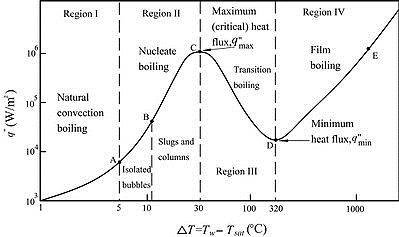
\includegraphics[width=0.5\textwidth]{./figure/400px-Boiling}
\caption{Boiling curveThe caption of a single sentence does not have period at the end}
\label{fig:boilingregime}
\end{figure}
%%%%%%%%%%%%%%%% end FIGURE 1 %%%%%%%%%%%%%%%%%%%

%%%%%%%%%%%%%%%% begin FIGURE 2 %%%%%%%%%%%%%%%%%%%
\begin{figure}[t]
\begin{center}
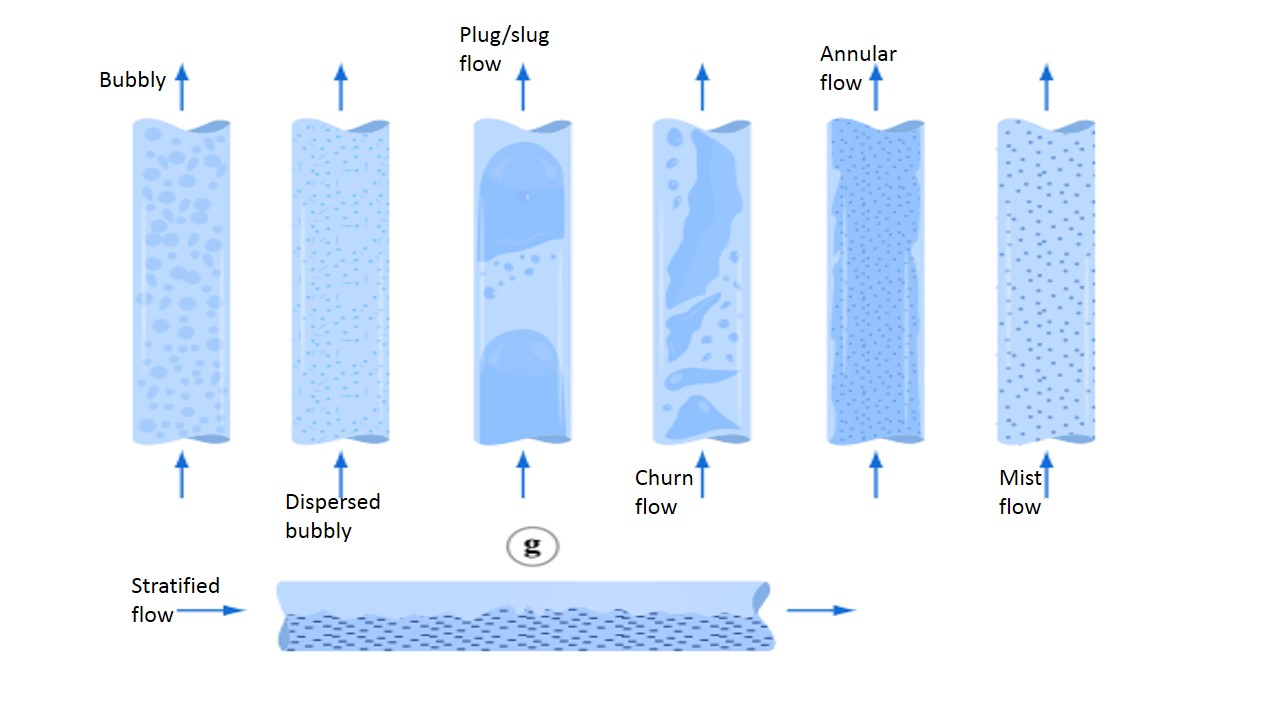
\includegraphics[width=0.75\textwidth]{./figure/flow_regime}
\end{center}
\caption{Flow Regime}
\label{fig:flowregime}
\end{figure}
%%%%%%%%%%%%%%%% end FIGURE %%%%%%%%%%%%%%%%%%

The Reynolds numbers used are

\begin{equation}
Re_{d_{p}} = \frac{\vec{v} d_p}{\nu_f}, ~~~ Re_{D_{\mathrm{pipe}}} = \frac{\vec{v} D_{\mathrm{pipe}}}{\nu_f}
\end{equation}

Again, the basic aim of this project is to compare the effectiveness of a metal foam when used inside a boiler as well as to find the sensitivity of the heat transfer based on the various properties of a metal foam. Based on the previous work done in this field, the following properties have been taken into consideration for the simulation and analysis of the model

% Citations?

\begin{itemize}
	\item Independent
		\begin{enumerate}
			\item $\rho_{cell} : [5,10,40] \mathrm{PPI}$
			\item $\phi_{porosity}= 0.97$, maximized
			\item $\dot{m} =63 \kilo\gram\per\second$, average
			\item $ q’’_(wall,max)=4.5 \kilo\watt\per\metre\squared$
			\item $ 0.025 < D_{\mathrm{pipe}} < .15 \metre$
			\item $ T_{in}=500K;P_{in} = 650 \kilo\pascal $
		\end{enumerate}
	\item Dependent
		\begin{enumerate}
			\item $100 < Re_{d_p} < 2.5 \times 3$
			\item $K_{permeability}= f(\Delta P)$
		\end{enumerate}
\end{itemize}

For the simulation of our model we have taken the ligament for the metal foam to be triangular and the overall shape of the cell to be tetrakiadecaheadron (14 phases - 8 equilateral triangle and 6 octagons).

\end{document}